\documentclass{article}

\usepackage{amsmath}
\usepackage{amssymb}
\usepackage{amsthm}
\usepackage{amsfonts}
\usepackage{graphicx}
\usepackage{xcolor}
\usepackage{dsfont}


\renewcommand{\vec}[1]{\mathbf{#1}}
\renewcommand{\r}[1]{\textcolor{blue}{#1}}
\newcommand{\Var}{\mathrm{Var}}
\newcommand{\Cov}{\mathrm{Cov}}
\renewcommand{\P}{\mathbb{P}}
\newcommand{\E}{\mathbb{E}}


\title{Econ 589 Econometrics: Problem set 1}

\begin{document}

\newtheorem{claim}{Claim}
\newtheorem{thm}{Theorem}
\newtheorem{mydef}{Definition}
\maketitle

\section{Question One.}


\section{Question Two.}


\section{Question Three.}
We consider the data generation process
\begin{equation} \r{y}_{i}=\theta_{0}+\log\r{u}_{i},\end{equation}
where $\r{u}_{i}$ is distributed according to a standard half-normal distribution. It is useful to note that $\r{u}_{i}\sim|Z|$ where $Z\sim N(0,1)$. To see this, note that for $u\geq0$, we have
\begin{equation}\begin{split} \P(\r{u}_{i}\leq u)&=\int_{0}^{u}f_{u}(t)dt \\
&= 2\int_{0}^{u}\phi(t)dt \\
&= 2\left(\int_{-\infty}^{u}\phi(t)dt-\int_{-\infty}^{0}\phi(t)dt\right) \\
&= 2\left(\Phi(u)-\frac{1}{2}\right)\\
&=2\Phi(u)-1,
\end{split}\end{equation}
and
\begin{equation}\begin{split}
\P(|\r{z}_{i}|\leq u) &= \P(\r{z}_{i}\in[-u,u])\\
&= \int_{-\infty}^{u}\phi(t)dt - \int_{-\infty}^{-u}\phi(t)dt\\
&=\Phi(t)-\Phi(-t)\\
&=\Phi(t)-(1-\Phi(t))\\
&=2\Phi(t)-1\\
&=\P(\r{u}_{i}\leq u),\end{split}\end{equation}
where the penultimate equality comes from the symmetry of the standard normal distribution.

We suppose that $\r{y}_{i}$ is observed and $\r{u}_{i}$ is not. 

As directed, we write
\begin{equation} \r{u}_{i}=\exp\left(\r{y}_{i}-\theta\right),\end{equation}
and define the log-likelihood
\begin{equation} \r{\hat{\theta}}=\text{argmax}_{\theta\in\Theta}\sum_{i\leq n}\log f_{u}\left(\exp\left(\r{y}_{i}-\theta\right)\right).\end{equation}

To investigate the properties of this estimator, we generated a data set with 1000 points. What we found is that the algorithm returned whatever the largest value of the range of values in the search was. This is because the objective of the MLE in this case is an increasing function of $\theta$. To see this, differentiate the objective with respect to $\theta$ to get
\begin{equation}\begin{split}
\r{l'}(\theta) &= \sum_{i\leq n} \frac{1}{f_{u}(\exp(y_{i}-\theta))}f'_{u}(\exp(y_{i}-\theta))(-\exp(y_{i}-\theta)) \\
&= \sum_{i\leq n}\frac{-\phi'(\exp(y_{i}-\theta))}{\phi(\exp(y_{i}-\theta))}\exp(y_{i}-\theta)\\
&>0,
\end{split}\end{equation}
where the inequality comes from noting that $\phi'>0$ for positive values (and all $\exp(y_{i}-\theta)$ are positive), $\phi>0$ for all values, and $\exp>0$ for all values. Since $\r{l'}>0$, $l$ is increasing, so the maximum is attained at the largest value of $\Theta$, or, more accurately, the maximum is obtained at $\max\Theta$ if this exists. In the case of unrestricted $\Theta$, we find that the algorithm will return the supremum. If we assume $\Theta=\mathbb{R}$ then, the MLE is $\infty$. Because the sample average of the objective is always increasing, the estimator is inconsistent.

To find a better estimator, we turn to GMM. We consider the moment condition
\begin{equation} \E[\exp(\r{y}_{i}-\theta_{0})-\E[\r{u}_{i}]]=0,\end{equation}
which is true since
\begin{equation} \E[\exp(\r{y}_{i}-\theta_{0})-\E[\r{u}_{i}]]=\E[\exp(\r{y}_{i}-\theta_{0})]-\E[\r{u}_{i}]=\E[\r{u}_{i}]-\E[\r{u}_{i}]=0.\end{equation}
Identification comes from noting that
\begin{equation}\begin{split} \E[\exp(\r{y}_{i}-\theta)]-\E[\r{u}_{i}]&=\E[\exp(\r{y}_{i}-\theta_{0}-(\theta-\theta_{0}))]-\E[\r{u}_{i}]\\
&=e^{-(\theta-\theta_{0})}\E[\exp(\r{y}_{i}-\theta_{0})]-\E[\r{u}_{i}]\\
&=e^{-(\theta-\theta_{0})}\E[\r{u}_{i}]-\E[\r{u}_{i}]\\
&=(e^{-(\theta-\theta_{0})}-1)\E[\r{u}_{i}].
\end{split}\end{equation}
Since $\r{u}_{i}$ is positive on a set of positive measure and negative nowhere, it must be the case that it has positive expectation, and hence the above expression is 0 if and only if $e^{-(\theta-\theta_{0})}=1$, which, since the exponential function is increasing, occurs if and only if $\theta=\theta_{0}$, and hence we have identification.

Since the expression inside the expectation operator is continuous, we have the desired features to ensure that the GMM estimator is consistent (if we assume a compact $\Theta$, which isn't so limiting since we can usually assume for economic reasons that the parameter will belong in some very large compact interval with a `guessed' upper and lower bound). Since the GMM estimator is consistent, it is significantly better than the MLE estimator. 






\section{Question Four.}


\section{Question Five.}
We consider data generated by 
\begin{equation} \r{y}_{i}=\theta_{0}\r{x}_{i}+\theta_{0}^{2}\r{a}_{i}+\r{u}_{i},\end{equation}
where it is known that $\r{x}_{i}$ and $\r{u}_{i}$ are independent of $\r{u}_{i}$, and that the mean of $\r{u}_{i}$ is 0. 

The true value of $\theta_{0}$ is 1, the means of $\r{x}_{i}$ and $\r{a}_{i}$ are 0, the variances are 1, and the correlation is 0.5; these facts are all considered unknown.

\subsection{Part (a).}
We wish to construct a moment condition such that $\theta_{0}$ is identified. We do this by noting that the independence of $\r{w}_{i}=(\r{x}_{i},\r{a}_{i})$ and $\r{u}_{i}$ gives us
\begin{equation} \E[\Gamma(\r{w}_{i})\r{u}_{i}]=\E[\Gamma(\r{w}_{i})]\E[\r{u}_{i}]=0,\end{equation}
where $\Gamma$ is some chosen instrument. This moment condition is then
\begin{equation}\label{eqn:mc5} \E[\Gamma(\r{w}_{i})(\r{y}_{i}-\theta_{0}\r{x}_{i}-\theta_{0}^{2}\r{a}_{i})]=0.\end{equation}

If we write $\Gamma(\r{w})=(\Gamma_{1}(\r{w}), \cdots, \Gamma_{m}(\r{w}))'$, then equation (\ref{eqn:mc5}) is a system of $m$ quadratic equations, which for generic $\theta$ are
\begin{equation} \theta^{2}\E[\Gamma_{k}(\r{w}_{i})\r{a}_{i}]+\theta\E[\Gamma_{k}(\r{w}_{i})\r{x}_{i}]-\E[\Gamma_{k}(\r{w}_{i})\r{y}_{i}]=0.\end{equation}
We know from our moment condition given by equation (\ref{eqn:mc5}) that $\theta_{0}$ satisfies this condition for each $k$. We wish this to be unique in doing so. 

Note that each equation in the system must have either 1 or 2 solutions. If any equation has 1 solution, then we are done, since $\theta=\theta_{0}$ must be this unique solution and hence uniquely solves the system. Suppose then that all of the equations in the system have two solutions. Again, by our moment condition it must be the case that for each of these, one of the two solutions is $\theta_{0}$. Therefore we have a set of $m$ quadratic equations all of which share a common root $\theta_{0}$. Because we assume that all of the equations have two roots, we are assuming that the coefficient on $\theta^{2}$ is non-zero in every equation, and hence we can rewrite our moment conditions as a set of $m$ monic quadratic equations which each are completely characterised by the root that is not $\theta_{0}$. All that is required is that one pair of these quadratic functions have a root that is not shared by them, and $\theta_{0}$ will be identified. 

Therefore, given $\Gamma$, all that is needed to show identification is to show that for some $j,l$, we have that 
\begin{equation} \begin{pmatrix} \frac{\E[\Gamma_{j}(\r{w}_{i})\r{x}_{i}]}{\E[\Gamma_{j}(\r{w}_{i})\r{a}_{i}]} & -\frac{\E[\Gamma_{j}(\r{w}_{i})\r{y}_{i}]}{\E[\Gamma_{j}(\r{w}_{i})\r{a}_{i}]}\end{pmatrix} \neq \begin{pmatrix} \frac{\E[\Gamma_{l}(\r{w}_{i})\r{x}_{i}]}{\E[\Gamma_{l}(\r{w}_{i})\r{a}_{i}]} & -\frac{\E[\Gamma_{l}(\r{w}_{i})\r{y}_{i}]}{\E[\Gamma_{l}(\r{w}_{i})\r{a}_{i}]}\end{pmatrix},\end{equation}
which is simply the claim that the monic polynomials earlier described have distinct coefficients and hence a distinct pair of roots; or show that one quadratic in the system is of the form $(\theta-\theta_{r})^{2}$ (and hence has only one root); or show that one of the equations is linear, that is, that there exists some $k$ for which $\E[\Gamma_{k}(\r{w}_{i})\r{a}_{i}]=0$. We will return to these conditions in the next part, but it suffices to say here that the likelihood of choosing an instrument such that the equations corresponding to each component are all the same equations is particularly low.

\subsection{Part (b).}
We wish to select the optimal instrument. Here we rely on our insight for GMM estimators more generally that the instrument that yields the efficient asymptotic variance is given by
\begin{equation} \Gamma(\r{w}_{i}) = B(\r{w}_{i})Q^{-1}(\r{w}_{i}),\end{equation}
where $B(w)=\E[\partial_{\theta}\r{b}(\theta_{0})'|\r{w}_{i}=w]$, with $\r{b}(\theta)=\r{y}-\theta\r{x}_{i}-\theta^{2}\r{a}_{i}$, and $Q(w)=\Var(\r{b}(\theta_{0})|\r{w}_{i}=w)$. We will calculate this instrument, and then check to verify that it identifies $\theta_{0}$ using the conditions discussed in the previous part.

\begin{equation}\begin{split} B(w) &= \E\left[\partial_{\theta}(\r{y}_{i}-\theta\r{x}_{i}-\theta^{2}\r{a}_{i})(\theta_{0})|\r{w}_{i}=w\right] \\ &= \E[-\r{x}_{i}-2\theta_{0}\r{a}_{i}|\r{w}_{i}=w]\\
&=-x-2\theta_{0}a.
\end{split}\end{equation}
For $Q$, note that the mean of $\r{b}(\theta_{0})$ is 0 as it is 
\begin{equation} \E[\r{u}_{i}|\r{w}_{i}=w]=\E[\r{u}_{i}]=0,\end{equation}
where the first equality comes from noting the independence of $\r{u}_{i}$ and $\r{w}_{i}$, and the second equality comes from noting that the mean of $\r{u}_{i}$ is 0. Therefore
\begin{equation}\begin{split} Q(w) &= \E\left[(\r{y}_{i}-\theta_{0}\r{x}_{i}-\theta_{0}^{2}\r{a}_{i})^{2}|\r{w}_{i}=w\right]\\
&=\E[\r{u}_{i}^{2}|\r{w}_{i}=w]\\
&=\sigma^{2},
\end{split}\end{equation}
where we have defined $\sigma^{2}$ to be the variance of the errors, which we have implicitly assumed by previous assumptions on $\r{u}_{i}$ satisfy homoskedasticity. Since the moment condition is set to 0, we can therefore drop the $\sigma^{2}$ so that our optimal instrument is 
\begin{equation} \Gamma(w) = x+2\theta_{0}a.
\end{equation}

Our moment condition is now
\begin{equation} \E[(\r{x}_{i}+2\theta_{0}\r{a}_{i})(\r{y}_{i}-\theta_{0}\r{x}_{i}-\theta_{0}^{2}\r{a}_{i})]=0.\end{equation}

This of course does not provide identification, since the instrument is a 1 dimensional quadratic (or cubic, depending on whether the $\theta_{0}$ in the instrument is taken as a variable rather than a constant). We therefore plot the data to determine that the positive root is that which should be taken.

\subsection{Part (c).}
We now want to compare the performance of three related estimators, defined as follows. $\r{\hat{\theta}}_{1}$ and $\r{\hat{\gamma}}$ solve
\begin{equation} \frac{1}{n}\sum_{i\leq n}\begin{pmatrix} \r{x}_{i}\\ \r{a}_{i}\end{pmatrix}(\r{y}_{i}-\r{\hat{\theta}}_{1}\r{x}_{i}-\r{\hat{\gamma}}\r{a}_{i})=0.\end{equation}
Note that this is two linear equations in two variables. We solve this to get
\begin{equation} \r{\hat{\theta}}_{1} = \frac{\r{\bar{ay}}-\r{\bar{a^{2}}}\r{\bar{xy}}}{\r{\bar{ax}}^{2}-\r{\bar{a^{2}}}\r{\bar{x^{2}}}},\end{equation}
where $\bar{\cdot}$ denotes the sample average of $\cdot$, so that, for example,
\begin{equation} \r{\bar{ay}}=\frac{1}{n}\sum_{i\leq n}\r{a}_{i}\r{y}_{i}.\end{equation}

The estimator $\r{\hat{\theta}}_{2}$ solves
\begin{equation} \frac{1}{n}\sum_{i\leq n} \r{z}_{i}(\r{\hat{\theta}}_{2})(\r{y}_{i}-\r{\hat{\theta}}_{2}\r{x}_{i}-\r{\hat{\theta}}_{2}^{2}\r{a}_{i})=0,\end{equation}
where $\r{z}_{i}$ is the optimal instrument from part (b). This is a cubic in $\r{\hat{\theta}}_{2}$, but of course, we want only one estimator. We therefore choose the largest root.

Finally, the estimator $\r{\hat{\theta}}_{3}$ is a two-stage estimator, that uses $\r{\hat{\theta}}_{1}$ to estimate the optimal instrument, so that $\r{\hat{\theta}}_{3}$ solves
\begin{equation} \frac{1}{n}\sum_{i\leq n}\r{z}_{i}(\r{\hat{\theta}}_{1})(\r{y}_{i}-\r{\hat{\theta}}_{3}\r{x}_{i}-\r{\hat{\theta}}_{3}^{2}\r{a}_{i})=0.\end{equation}
This is quadratic in our parameter, so we take the positive root, unless that proves to be badly behaved.

What we find when we run the code is that, regardless of variance, $\r{\hat{\theta}}_{2}$ always tracks $\r{\hat{\theta}}_{3}$ incredibly tightly, lying slightly above to an incredibly small degree, such that the resulting difference appears to be very stochastic and always positive. Further, we find that these two estimators are significantly better estimators than $\r{\hat{\theta}}_{1}$ in convergence rate.

The latter conclusion is hardly surprising, as these estimators are either the optimal estimator of this type or a two stage approximation of that estimator. We therefore turn our attention to the high degree of correlation between $\r{\hat{\theta}}_{2}$ and $\r{\hat{\theta}}_{3}$.

\begin{figure}[h]
\centering
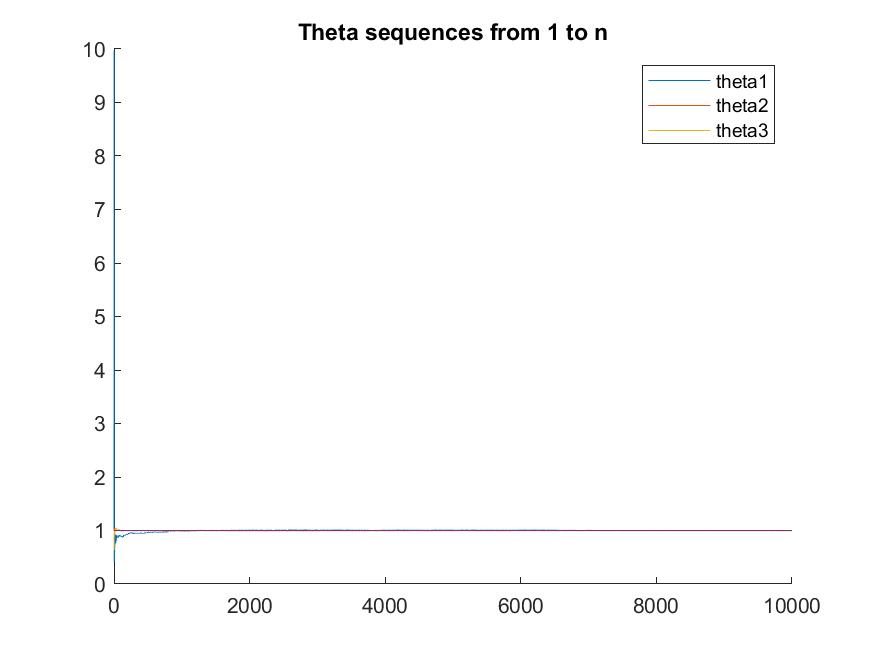
\includegraphics[width=13cm]{q5partc1.jpeg}
\caption{The estimators over a run of 10000 data points.}
\label{fig:5c1}
\end{figure} 

\begin{figure}[h]
\centering
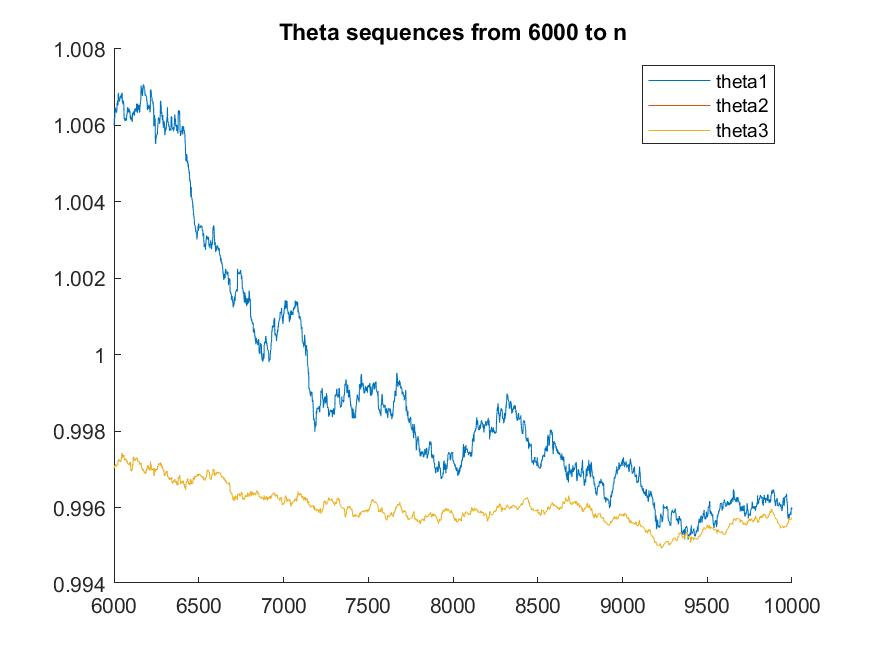
\includegraphics[width=13cm]{q5partc2.jpeg}
\caption{The estimators over a run of 10000 data points, from the 6000th point onwards.}
\label{fig:5c2}
\end{figure} 


\begin{figure}[h]
\centering
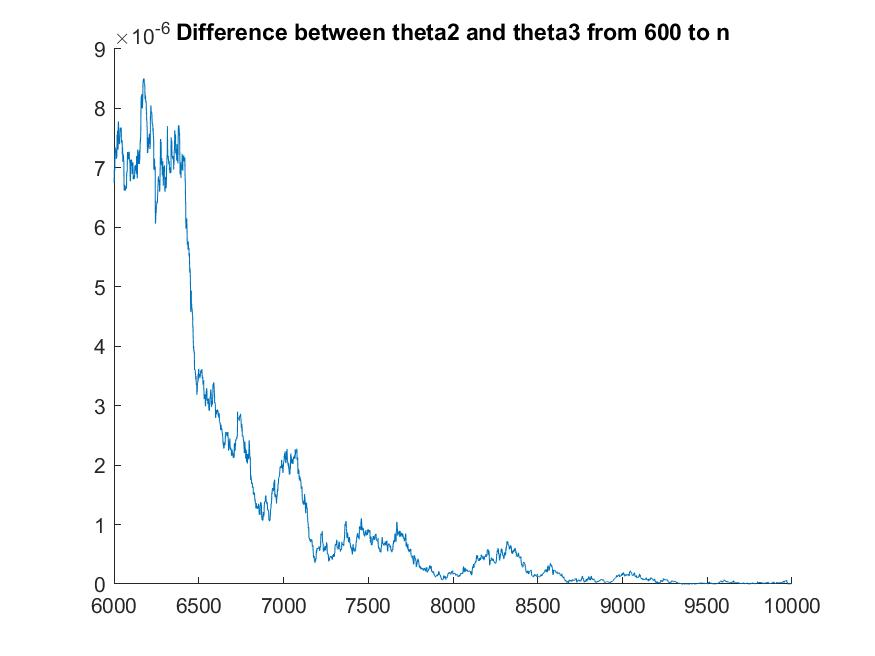
\includegraphics[width=13cm]{q5partc3.jpeg}
\caption{The difference between $\r{\hat{\theta}}_{2}$ and $\r{\hat{\theta}}_{3}$, with the latter always slightly lower than the former, but to an incredibly small degree, indicating an incredibly high degree of correlation.}
\label{fig:5c3}
\end{figure} 





\section{Question Six.}


\section{Question Seven.}
We have two distributions, $\r{l}_{i}=\exp(\r{Z}_{l})$, where $\r{Z}_{l}\sim N(\mu_{l},\sigma_{l}^{2})$ and $\r{b}_{i}=\exp(\r{Z}_{b})$ where $\r{Z}_{b}\sim N(\mu_{b},\sigma_{b}^{2})$, and we are interested in finding $\lambda_{0}=\E[\r{l}_{i}]$, $\beta_{0}=\E[\r{b}_{i}],$ and $\Var(\r{l}_{i})=\Var(\r{b}_{i})=\sigma_{0}^{2}$, when we observe $\r{a}_{i}=\r{l}_{i}\r{b}_{i}$. We proceed by using MLE.

\subsection{Part (a).}
We wish to find the loglikelihood function for this problem. First we need to find the distribution of $\r{a}_{i}$. We let $Z_{i}$ denote independent standard normal distributions.
\begin{equation}\begin{split}
\r{a}_{i} &= \r{l}_{i}\r{b}_{i} = \exp\left(\sigma_{l}\r{Z}_{1}+\mu_{l}\right)\exp\left(\sigma_{b}\r{Z}_{2}+\mu_{b}\right)\\
&=\exp\left(\sigma_{l}\r{Z}_{1}+\sigma_{b}\r{Z}_{2}+(\mu_{l}+\mu_{b})\right).\end{split}\end{equation}
We know that 
\begin{equation}\sigma_{l}\r{Z}_{1}+\sigma_{b}\r{Z}_{2}+(\mu_{l}+\mu_{b})\sim N(\mu,\sigma_{a}^{2})\end{equation}
where 
\begin{equation} \mu=\mu_{l}+\mu_{b}, \; \; \sigma_{a}^{2}=\sigma_{l}^{2}+\sigma_{b}^{2},\end{equation}
and hence 
\begin{equation}\r{a}_{i}\sim\exp(N(\mu,\sigma_{a}^{2})).\end{equation}
That is, $\r{a}_{i}$ is log-normal with parameters $\mu=\mu_{l}+\mu_{b}$ and $\sigma_{a}^{2}=\sigma_{l}^{2}+\sigma_{b}^{2}$. We write $\r{a}_{i}=\exp(\r{Z}_{a})$ where $\r{Z}_{a}\sim N(\mu,\sigma_{a}^{2})$.

As such, we now wish to find the likelihood distribution for i.i.d. lognormally distributed data. We denote the cdf and pdf by $F$ and $f$ respectively, and find that
\begin{equation}\begin{split}
F(a;\mu,\sigma_{a}^{2}) &= \P(\r{a}_{i}\leq a)=\P(\exp(\r{Z}_{a})\leq a) \\
&= \P(\r{Z}_{a}\leq \log a) = \P(\sigma_{a}\r{Z}_{3}+\mu \leq \log a)\\
&=\P\left(\r{Z}_{3}\leq \frac{\log a-\mu}{\sigma_{a}}\right)\\
&=\Phi\left(\frac{\log a-\mu}{\sigma_{a}}\right),
\end{split}\end{equation}
so that differentiating with respect to $a$ gives
\begin{equation}f(a;\mu,\sigma_{a}^{2}) = \phi\left(\frac{\log a -\mu}{\sigma_{a}}\right)\cdot\frac{1}{\sigma_{a}a}.\end{equation}

Our likelihood function $L$ is therefore
\begin{equation} \r{L}(\mu,\sigma_{a}^{2}) = \prod_{i\leq n}\phi\left(\frac{\log a_{i} -\mu}{\sigma_{a}}\right)\cdot\frac{1}{\sigma_{a}a_{i}},\end{equation}
which implies that our log-likelihood function is
\begin{equation}
\r{l}(\mu,\sigma_{a}^{2}) = \sum_{i\leq n}\left(\log\phi\left(\frac{\log{a_{i}}-\mu}{\sigma_{a}}\right)-\log{\sigma_{a}}-\log{a_{i}}\right).\end{equation}

Since we are maximising $\mu,\sigma_{a}^{2}$, the last term here is a constant, so we ignore this and divide through by $n$ to get the sample objective
\begin{equation} \r{\hat{Q}}(\mu,\sigma_{a}^{2}) = \frac{1}{n}\sum_{i\leq n}\left(\log{\phi\left(\frac{\log\r{a}_{i}-\mu}{\sigma_{a}}\right)}-\log{\sigma_{a}}\right).
\end{equation}
Using our expression for $\mu$ and $\sigma_{a}^{2}$ in terms of $\mu_{l}$, $\mu_{b}$, $\sigma_{l}^{2}$, and $\sigma_{b}^{2}$, we get
\begin{equation}\r{\hat{Q}}(\mu_{l},\mu_{b},\sigma_{l}^{2}+\sigma_{b}^{2}) = \frac{1}{n}\sum_{i\leq n}\left(\log{\phi\left(\frac{\log\r{a}_{i}-(\mu_{l}+\mu_{b})}{\sqrt{\sigma_{l}^{2}+\sigma_{b}^{2}}}\right)}-\frac{1}{2}\log(\sigma_{l}^{2}+\sigma_{b}^{2})\right).\end{equation}

Finally, we note that we wish to find $\lambda_{0}$, $\beta_{0}$, and $\sigma_{0}^{2}$, so we find expressions for $\mu_{l}$, $\mu_{b}$, $\sigma_{l}^{2}$, and $\sigma_{b}^{2}$ in terms of these parameters.

Note that by properties of the log-normal distribution, we have
\begin{equation}\label{eqn:mean} \E[\r{l}_{i}]=\lambda_{0}=\exp\left(\mu_{l}+\frac{\sigma_{l}^{2}}{2}\right), \end{equation}
\begin{equation} \Var(\r{l}_{i})=\sigma_{0}^{2} =(\exp(\sigma_{l}^{2})-1)(2\mu_{l}+\sigma_{l}^{2}).\end{equation}
We use equation (\ref{eqn:mean}) to express $\sigma_{l}^{2}$ in terms of $\mu_{l}$ to get
\begin{equation} \sigma_{l}^{2} = 2(\log\lambda_{0}-\mu_{l}).\end{equation}
Substituting this into the equation given by the variance and rearranging, we find that
\begin{equation}\mu_{l}=\log\lambda_{0}-\frac{1}{2}\log\left(\frac{\sigma_{0}^{2}}{\exp(2\log\lambda_{0})}+1\right),\end{equation}
and
\begin{equation}\sigma_{l}^{2} = \log\left(\frac{\sigma_{0}^{2}}{\exp(2\log\lambda_{0})}+1\right).\end{equation}
Similarly, for $b$ we have
\begin{equation} \mu_{b} = \log\beta_{0}-\frac{1}{2}\log\left(\frac{\sigma_{0}^{2}}{\exp(2\log\beta_{0})}+1\right),\end{equation}
and
\begin{equation}\sigma_{b}^{2} = \log\left(\frac{\sigma_{0}^{2}}{\exp(2\log\beta_{0})}+1\right).\end{equation}
We therefore have the sample objective function
\begin{equation}\begin{split}
\r{\hat{Q}}(\lambda,\beta,\sigma) = \frac{1}{n}&\sum_{i\leq n}\log{\phi\left(\frac{\log\r{a}_{i}-(\log\lambda+\log\beta)+\frac{1}{2}\left(\log\left(\frac{\sigma^{2}}{\exp(2\log\lambda)}+1\right)+\log\left(\frac{\sigma^{2}}{\exp(2\log\beta)}+1\right)\right)}{\sqrt{\log\left(\frac{\sigma^{2}}{\exp(2\log\lambda)}+1\right)\log\left(\frac{\sigma^{2}}{\exp(2\log\beta)}+1\right)}}\right)}\\
&-\frac{1}{2n}\sum_{i\leq n}\log\left(\log\left(\frac{\sigma^{2}}{\exp(2\log\lambda)}+1\right)+\log\left(\frac{\sigma^{2}}{\exp(2\log\beta)}+1\right)\right).
\end{split}\end{equation}



\subsection{Part (b).}
Given a dataset, we now use our sample objective in order to estimate the desired means and variance. The estimate we get is $\lambda_{0}=206.3425$, $\beta_{0}=80.4814$, $\sigma_{0}=0.5691$.

I would, however, just send an RA with clearer instructions before buying a table cloth because I am not at all convinced that this code is robust.

\subsection{Part (c).} 
We now fix $\lambda_{0}=200$, $\beta=80$, and let the variance run through $0.5$ to $50$ in incerements of 0.5. We calculate the root mean squared error of the area against the variance. We subsequently then checked values from 0.5 to 2 in increments of 0.05. It gave us very little.

\begin{figure}[h]
\centering
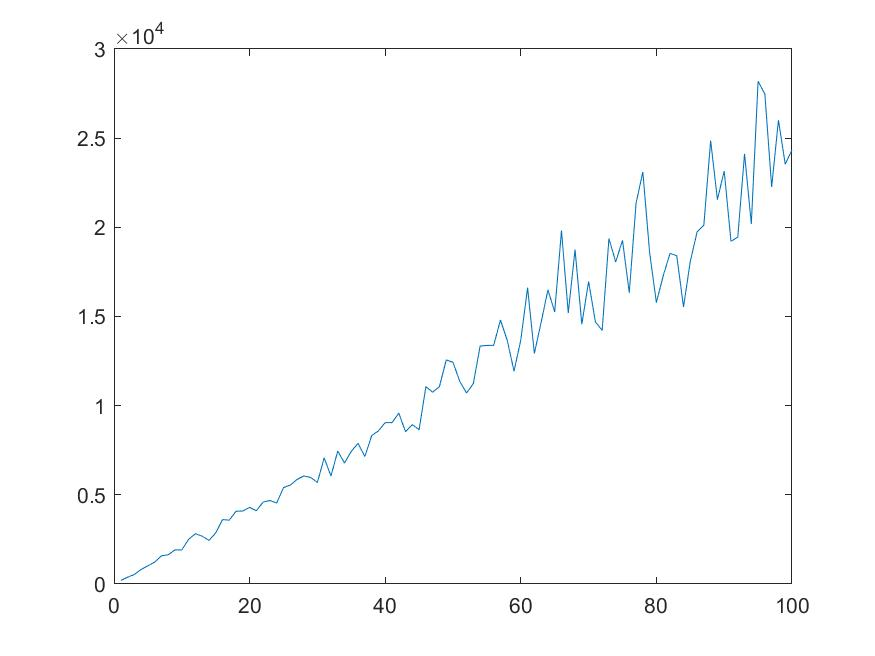
\includegraphics[width=13cm]{q7partc1.jpeg}
\end{figure} 
\begin{figure}[h]
\centering
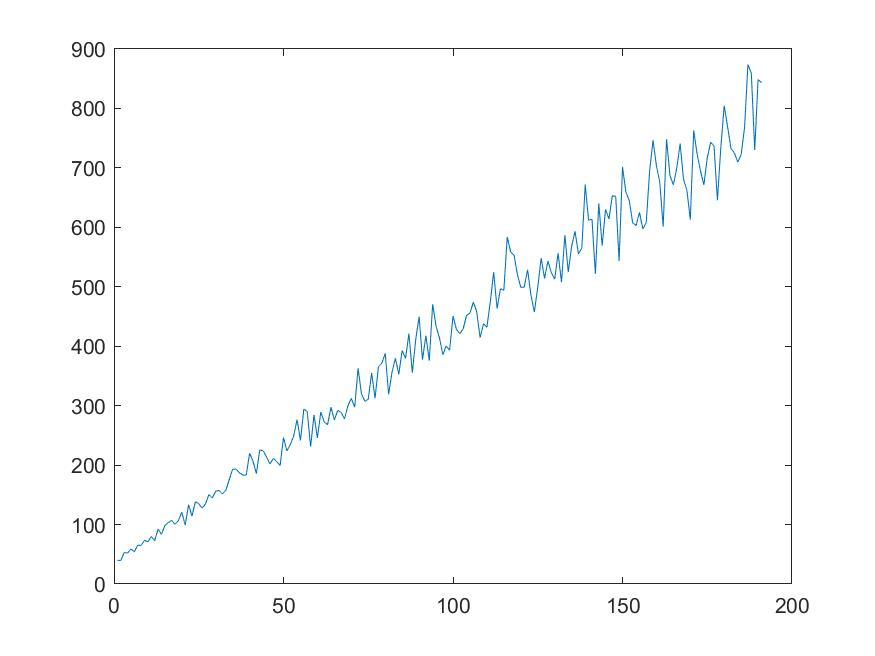
\includegraphics[width=13cm]{q7partc2.jpeg}
\end{figure} 





\section{Question Eight.}
We consider two random variables with joint distribution function
\begin{equation} F(x,y)=\Phi(x)\Phi(y)(1-0.5\Phi(-x)\Phi(-y)).\end{equation}

\subsection{Part (a).}
We first verify that this is in fact a distribution function. Note that as $x$ and $y$ tend to infinity, $F$ tends to $1\cdot1(1-0.5\cdot0\cdot0)=1$. As $x$ and $y$ tend to $-\infty$, $\Phi(x)$ tends to 0, so $F$ tends to 0. The distribution is clearly continuous and hence is right-continuous. Finally, the term $\Phi(x)\Phi(y)$ is increasing in both $x$ and $y$, and $(1-0.5\Phi(-x)\Phi(-y))$ is increasing in $x$ and $y$, and hence $F$ is increasing in $x$ and $y$, and hence is a distribution function.

\subsection{Part (b).}
We now consider the marginal distributions. For this, we let $y$ tend to $\infty$, and see that
\begin{equation} F_{X}(x)=\lim_{y\to\infty}F(x,y)=\Phi(x).\end{equation}
Similarly, then, $F_{Y}(y)=\Phi(y)$. That is, $\r{x}$ and $\r{y}$ are both distributed as standard normal random variables.

\subsection{Part (c).}
We wish to draw the joint density function of $\r{x},\r{y}$, by which I mean, we wish to get matlab to do that, so we calculate the joint pdf $f_{XY}$:
\begin{equation}\begin{split}
&f_{XY}(x,y) = \frac{\partial^{2}F}{\partial y \partial x}\\
&= \frac{\partial}{\partial y}\left(\phi(x)\Phi(y)(1-0.5\Phi(-x)\Phi(-y))+0.5\Phi(x)\Phi(y)\Phi(-y)\phi(-x)\right)\\
&=\phi(x)((\phi(y)(1-0.5\Phi(-x)\Phi(-y))+0.5\Phi(y)\Phi(-x)\phi(-y)))\\&+0.5\Phi(x)\phi(y)\phi(-x)\Phi(-y)-0.5\Phi(x)\Phi(y)\phi(-y)\phi(-x)\\
&= \phi(x)\phi(y)(1-0.5\Phi(-x)\Phi(-y))+0.5\phi(x)\phi(-y)\Phi(-x)\Phi(y)\\&+0.5\Phi(x)\phi(y)\phi(-x)\Phi(-y)-0.5\phi(-x)\phi(-y)\Phi(x)\Phi(y)
\end{split}\end{equation}

This produces the following plot.
\begin{figure}[h]
\centering
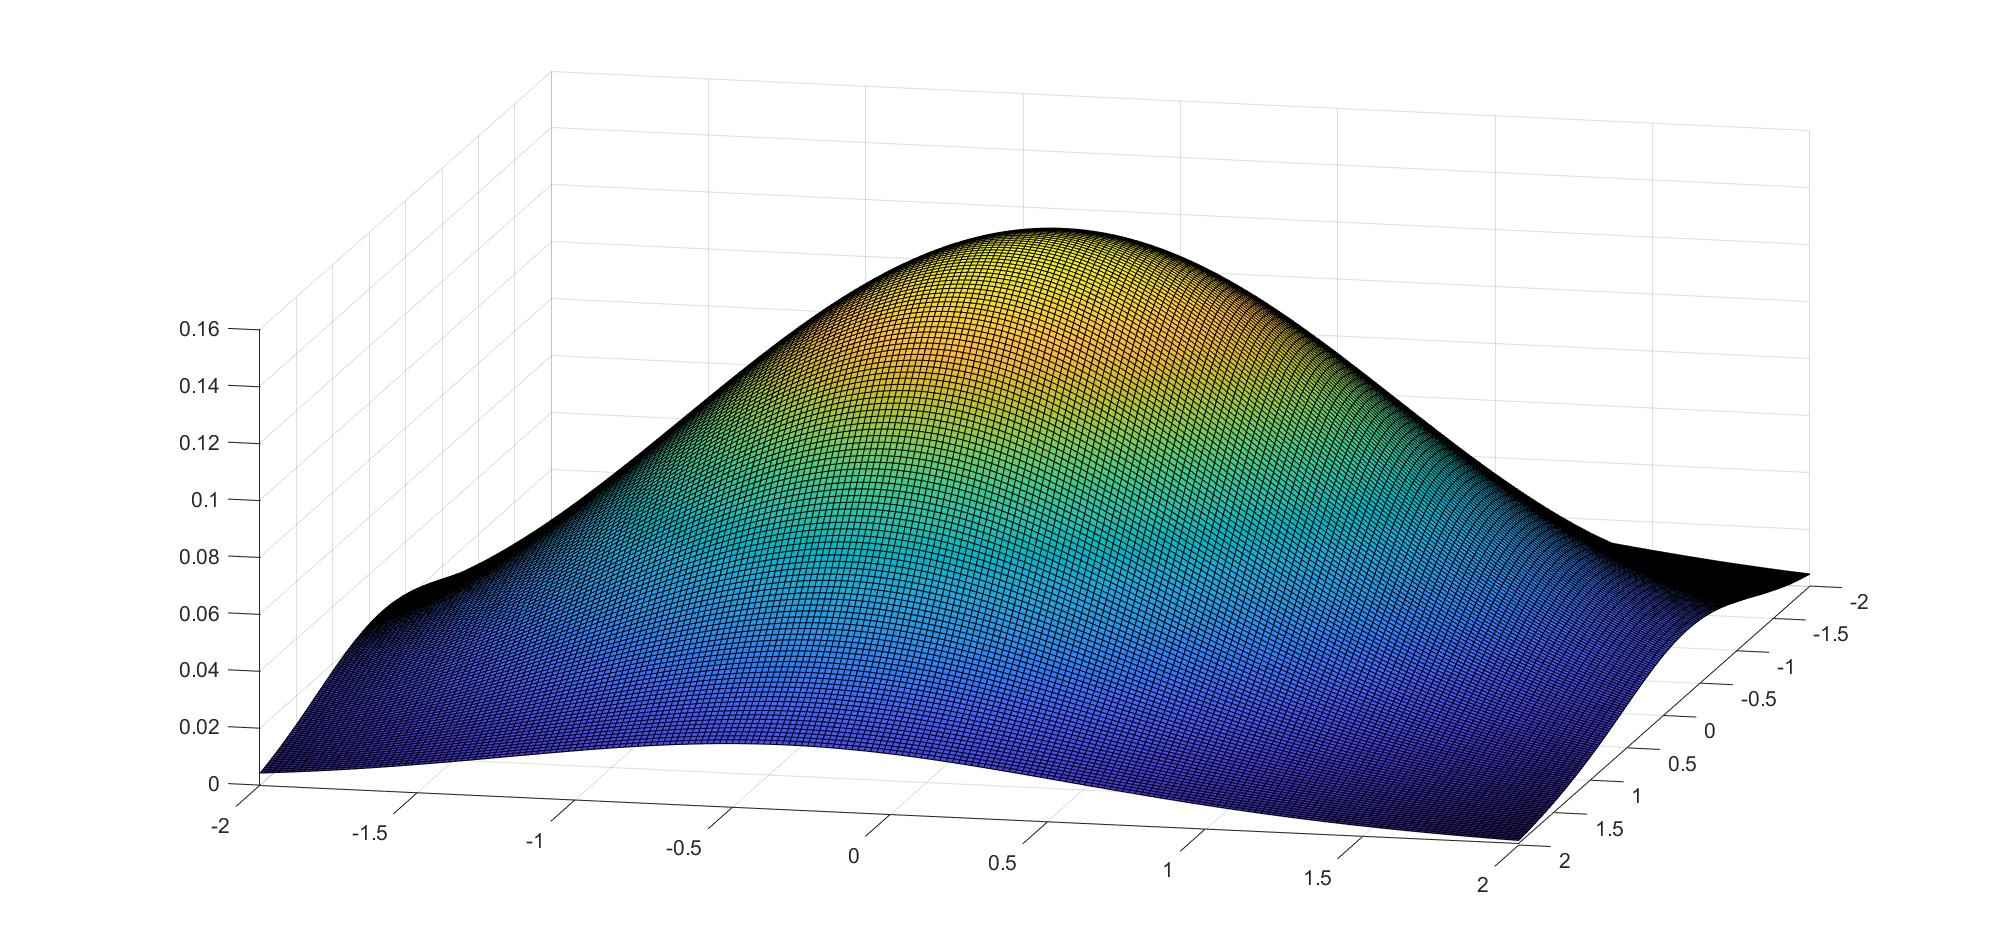
\includegraphics[width=13cm]{q8partc.jpeg}
\caption{The joint distribution of $\r{x}$ and $\r{y}$ plot over $[-2,2]\times[-2,2]$ with grid points spaced 0.02 apart.}
\label{fig:8c}
\end{figure} 

\subsection{Part (d).}
We wish to plot various distributions of $\r{x}$ conditional on $\r{y}$. For this, we note that
\begin{equation} f_{X|Y}(x|y)=\frac{f_{XY}(x,y)}{f_{Y}(y)}.\end{equation}
Here of course, $f_{Y}(y) = \phi(y)$, from part (b). We plot this for $y=0,\pm1,\pm0.5$ below

\begin{figure}[h]
\centering
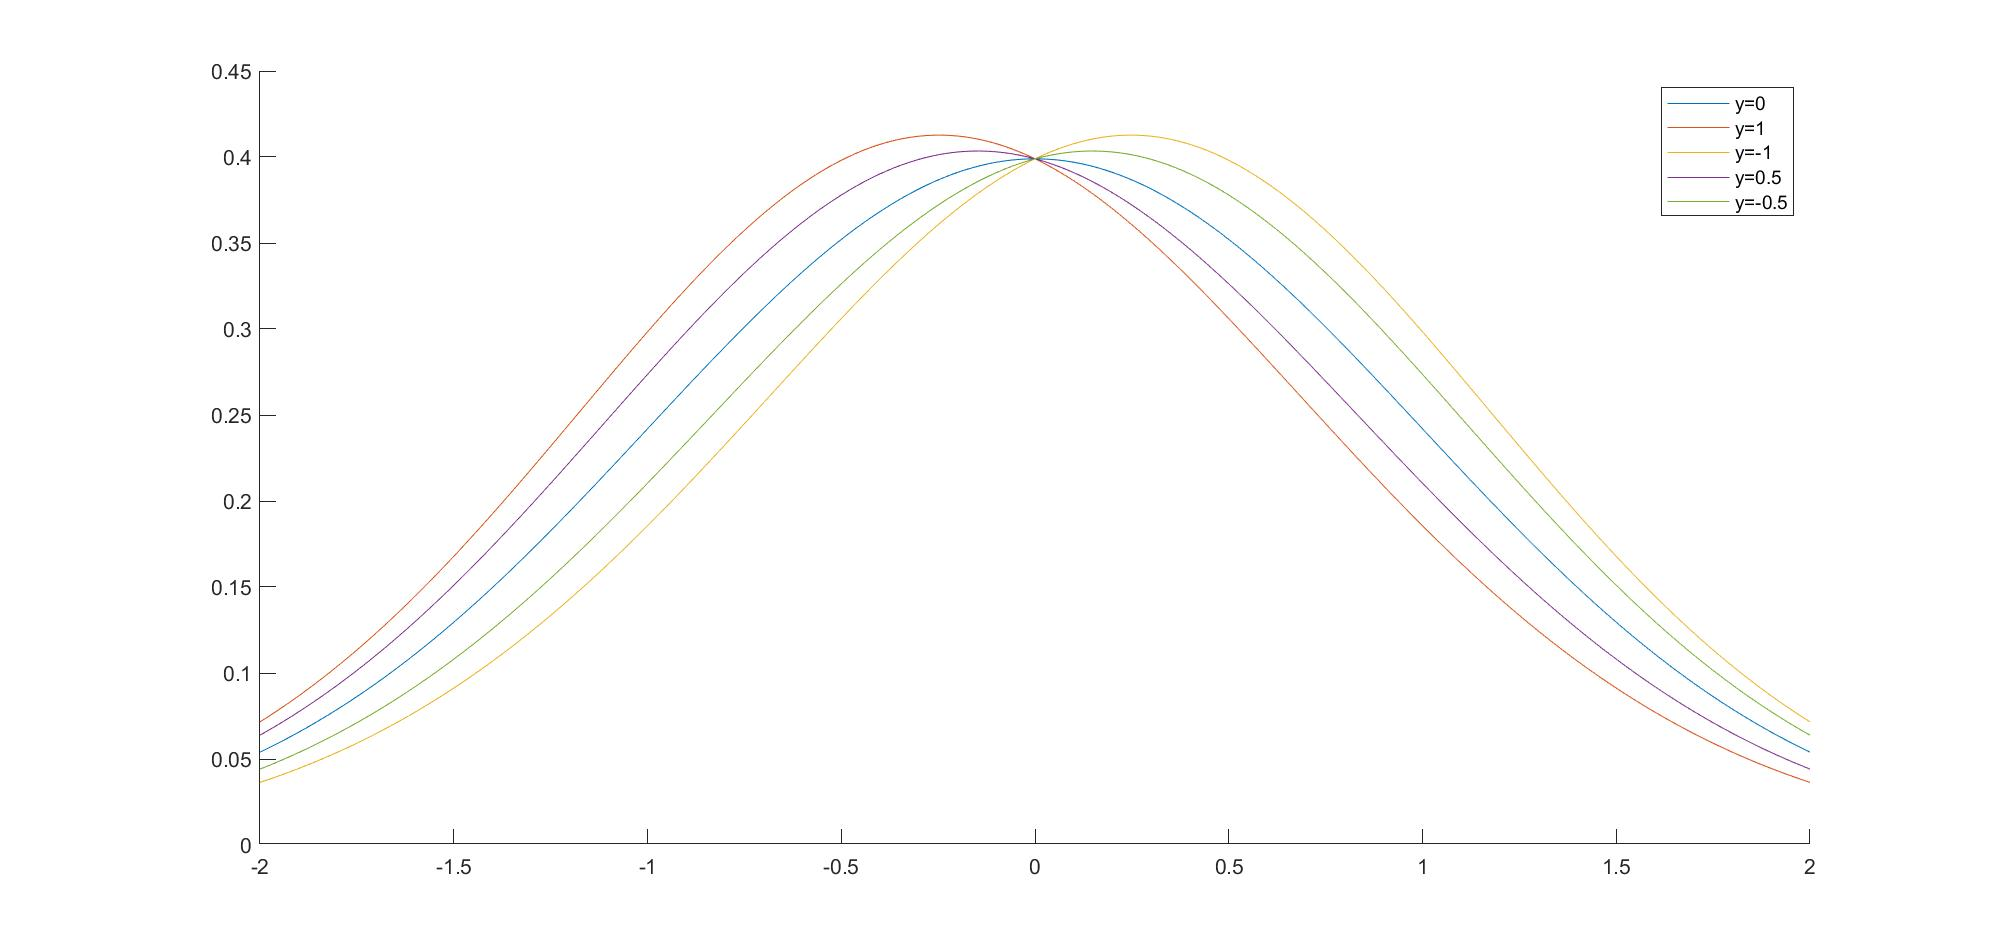
\includegraphics[width=13cm]{q8partd.jpeg}
\caption{The conditional distribution of $\r{x}$ and $\r{y}$ plot over $[-2,2]$ with grid points spaced 0.02 apart, for $y=0,\pm1,\pm0.5$.}
\label{fig:8d}
\end{figure} 

\subsection{Part (f).}
We repeat the exercise with the random variables now given by the distribution
\begin{equation} f_{XY}=c\phi(x)\phi(y)(1+|x||y|\mathds{1}\{\max\{|x|,|y|\}<1\}),\end{equation}
where $c$ is a normalisation constant.
\subsubsection{Part (a).}
Clearly $f$ is non-negative everywhere. Further, it is clear that the integral is bounded:
\begin{equation}\begin{split}
\int f_{XY}(x,y)dxdy &=c\int\phi(x)\phi(y)dxdy + c\int_{-1}^{1}\int_{-1}^{1}|xy|\phi(x)\phi(y)dxdy\\
&=c+c\int_{-1}^{1}\int_{-1}^{1}|xy|\phi(x)\phi(y)dxdy
\end{split}\end{equation}
This integral is of a continuous function on a compact space, and hence is finite. We can therefore choose $c$ such that the integral of the density over $\mathbb{R}^{2}$ is 1, and hence $f_{XY}$ characterises a distribution.

\subsubsection{Part (b).}
We now wish to consider the marginal distributions, which we do by integrating our density over $y\in(-\infty,\infty)$. 
\begin{equation}\begin{split}
f_{X}(x) &= \int_{-\infty}^{\infty}f_{XY}(x,y)dy \\
&= c\phi(x)\left(\int_{-\infty}^{\infty}\phi(y)(1+|x||y|\mathds{1}\{\max\{|x|,|y|\}<1\})dy\right)\\
&= c\phi(x)\left(1+|x|\mathds{1}\{|x|<1\}\int_{-1}^{1}|y|\phi(y)dy\right)\\
&=c\phi(x)\left(1+2|x|\mathds{1}\{|x|<1\}\int_{0}^{1}y\phi(y)dy\right)
\end{split}\end{equation}

We handle this last integral using integration by parts, so that
\begin{equation}\begin{split}
\int_{0}^{1}y\phi(y)dy &= \left[y\Phi(y)\right]_{0}^{1}-\int_{0}^{1}\Phi(y)dy\\
&= \Phi(1)-\left[y^{2}\Phi(y)+\phi(y)\right]_{0}^{1}\\
&=\Phi(1) - \Phi(1) - \phi(1)+\phi(0)\\
&= \phi(0)-\phi(1)\\
&= \frac{1}{\sqrt{2\pi}}(1-e^{-\frac{1}{2}}).
\end{split}\end{equation}

We therefore have that
\begin{equation} f_{X}(x) = c\phi(x)\left(1+\frac{\sqrt{2}|x|}{\sqrt{\pi}}\mathds{1}\{|x|<1\}(1-e^{-\frac{1}{2}})\right).\end{equation}

By symmetry, we have
\begin{equation} f_{Y}(y) = c\phi(y)\left(1+\frac{\sqrt{2}|y|}{\sqrt{\pi}}\mathds{1}\{|x|<1\}(1-e^{-\frac{1}{2}})\right).\end{equation}

Given the above calculation, we can now in fact find the value of $c$. 
\begin{equation}\begin{split}
\int f_{XY}(x,y)dxdy&=c\left(1+4\left(\int_{0}^{1}x\phi(x)dx\right)^{2}\right)\\
&= c\left(1+\frac{2}{\pi}(1-e^{-\frac{1}{2}})^{2}\right)\\
&=1,
\end{split}\end{equation}
where the last equality comes from noting that $c$ normalises the distribution, and hence
\begin{equation} c=\left(1+\frac{2}{\pi}(1-e^{-\frac{1}{2}})^{2}\right)^{-1}.\end{equation}

\subsubsection{Part (c).}
We now plot our pdf.

\begin{figure}[h]
\centering
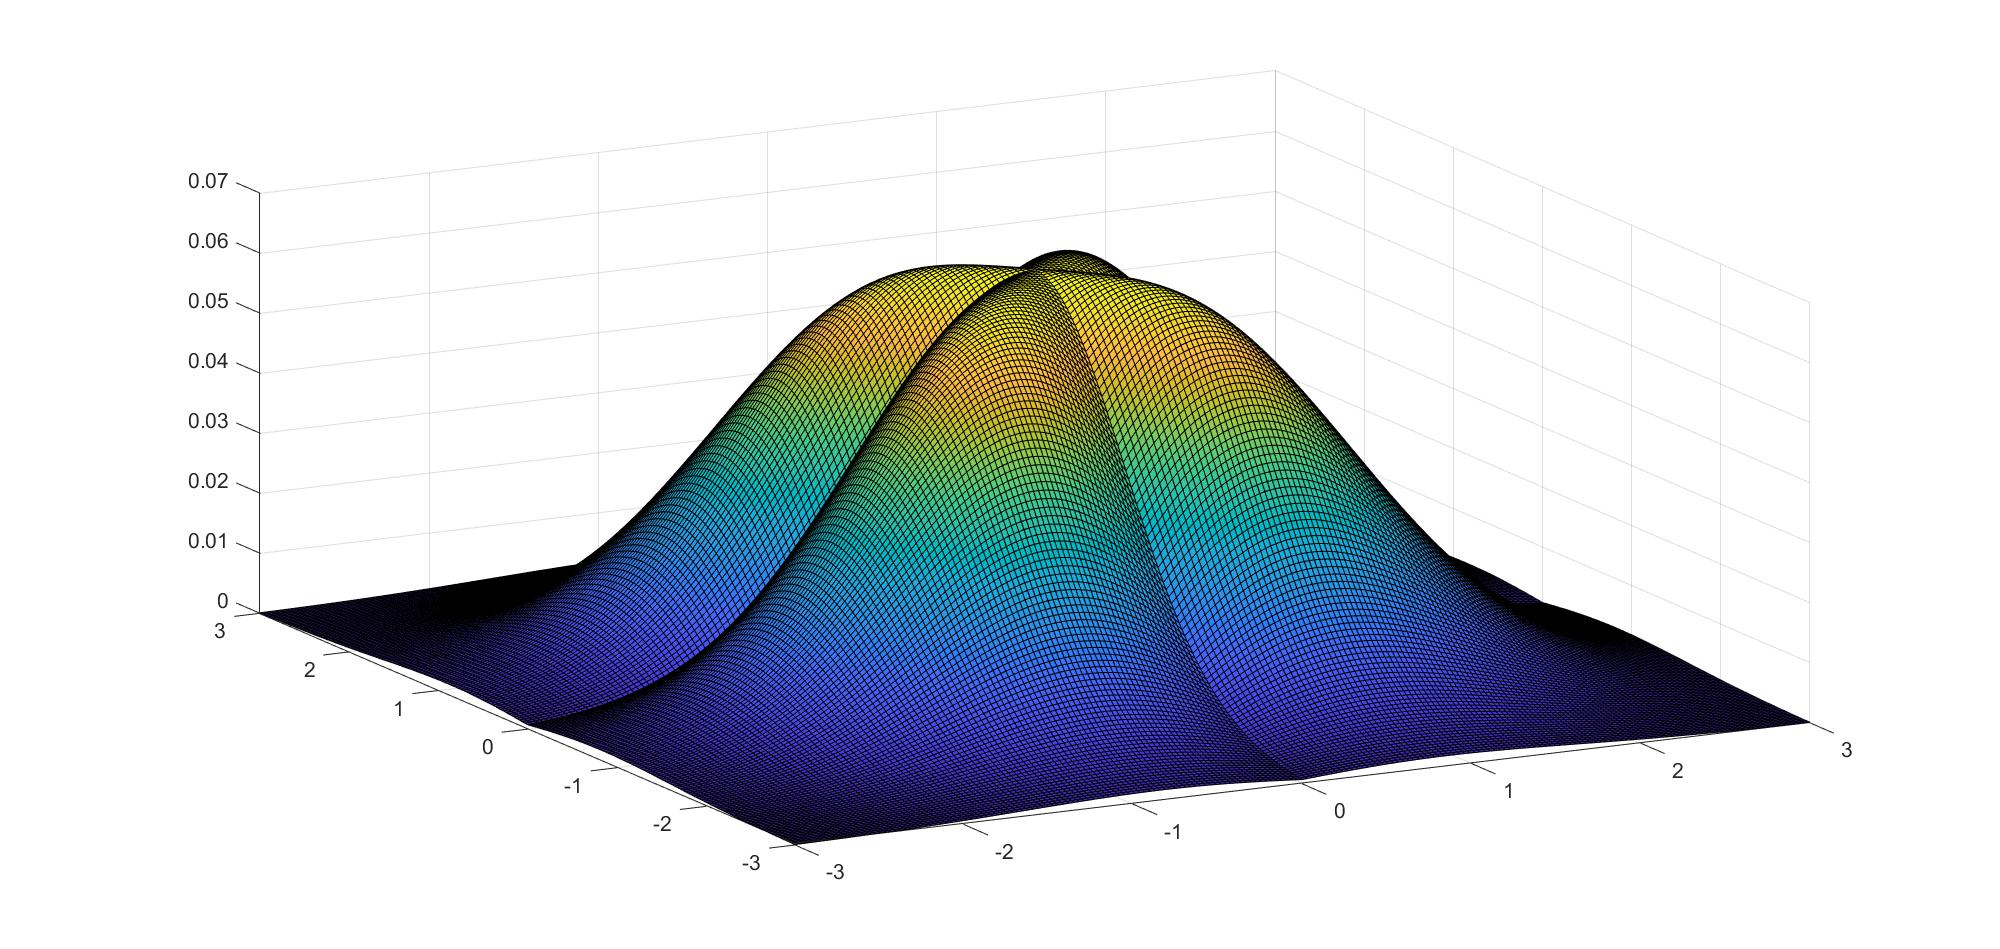
\includegraphics[width=13cm]{q8fpartc.jpeg}
\caption{The joint distribution of $\r{x}$ and $\r{y}$ plot over $[-3,3]\times[-3,3]$ with grid points spaced 0.03 apart.}
\label{fig:8fc}
\end{figure} 

\subsubsection{Part (d).}
We now plot the conditional distributions, given $y=0,\pm1,\pm0.5$.


\begin{figure}[h]
\centering
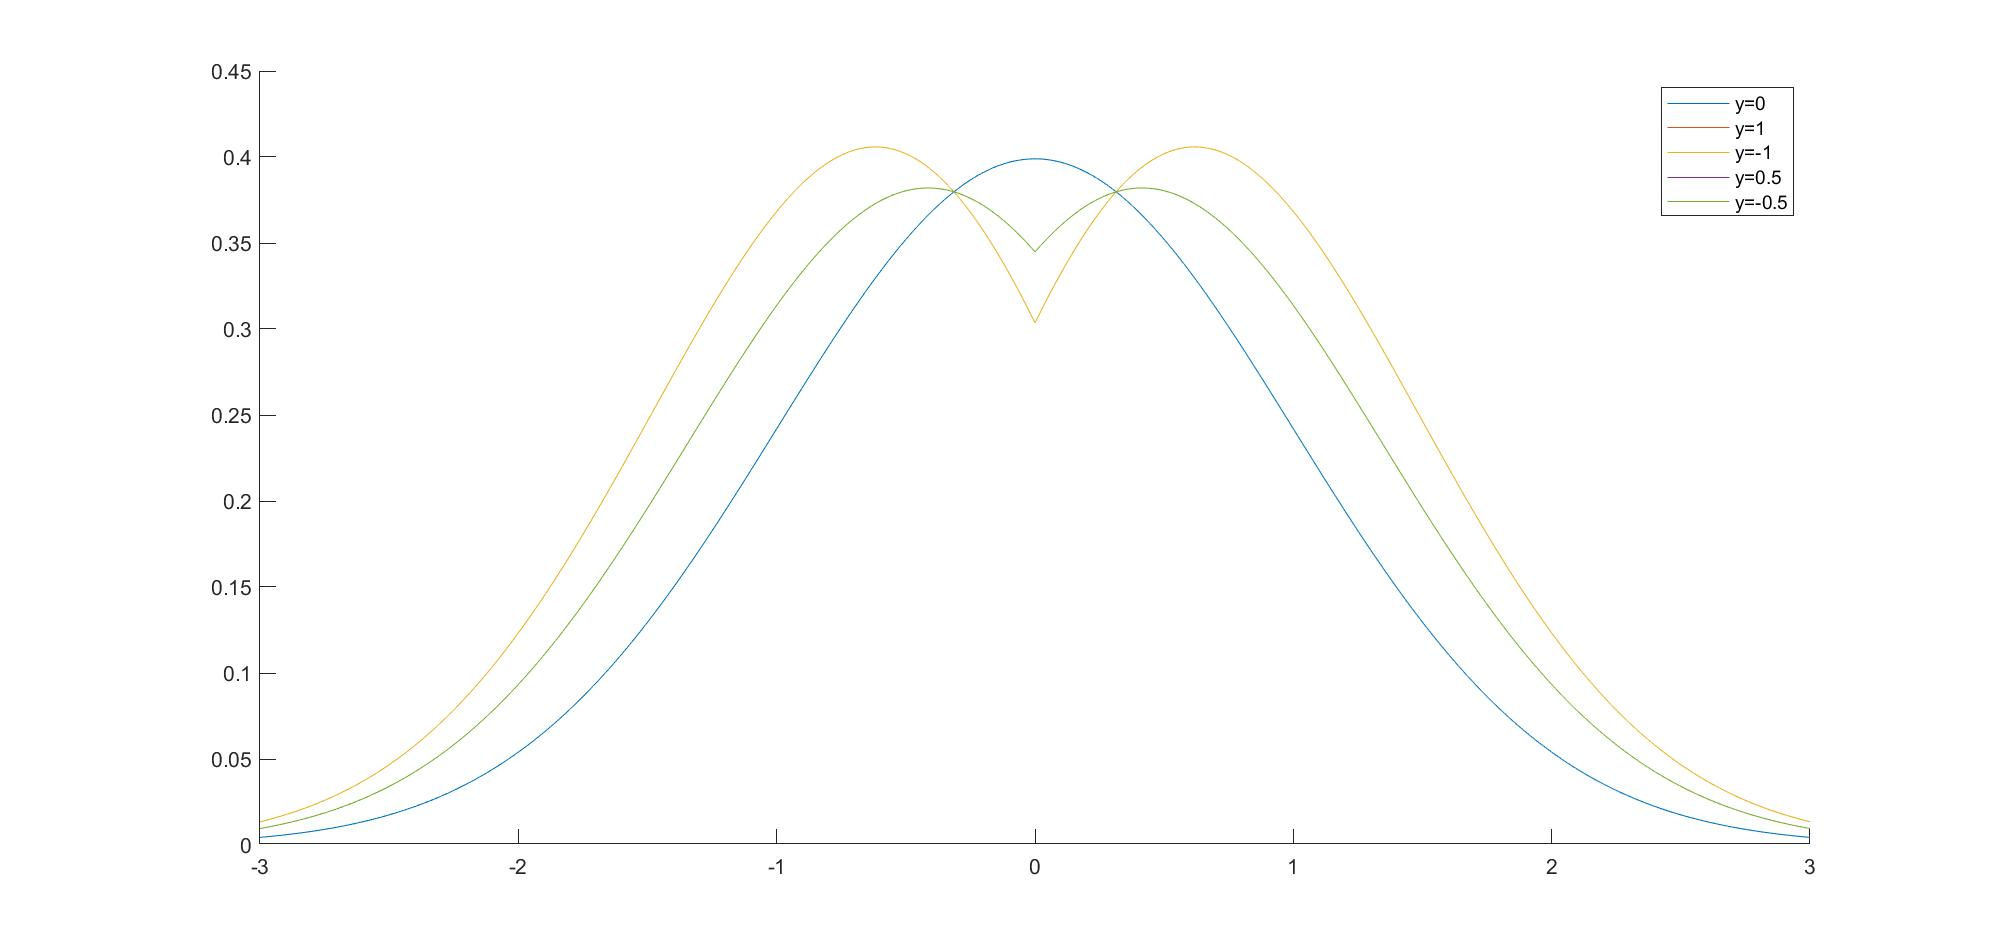
\includegraphics[width=13cm]{q8fpartd.jpeg}
\caption{The conditional distribution of $\r{x}$ and $\r{y}$ plot over $[-3,3]$ with grid points spaced 0.03 apart, for $y=0,\pm1,\pm0.5$.}
\label{fig:8fd}
\end{figure} 







\end{document}